\documentclass[addpoints]{physlabs}

\labtitle{Thermal and Mechanical Energy}
\labnum{5}
\labnumroman{V}
\course{PHYSICS 113 - 121 - 181}
\coursesubtitle{General Physics I and Mechanics}
\date{\today}

\usetikzlibrary{patterns, angles, quotes, shapes, shapes.geometric, arrows.meta}

% Gray table column type
\newcolumntype{g}{>{\columncolor{gray!20}}c}

\begin{document}

\maketitle

% PRELAB SECTION
\begin{prelab}

    \filbreak
    \question[1] A \qty{90}{\kilo\gram} person jumps from a \qty{30}{\meter} tower into a tub of water with a volume of \qty{5}{\meter^3} initially at \qty{20}{\celsius}. Assuming that all of the work done by the person is converted to heat the water, what is the final temperature of the water? Note: It is helpful to first find the work done by the person on the water tub and then the amount of heat equivalent to that work. Make sure you have the correct value for the mass of the water, and include units.
    %
    \begin{solution}[8cm]
        By the work-energy theorem, the work done is the change in kinetic energy of the person, which is equal to the change in potential energy during the fall. We can then set this equal to the change in heat of the tub to find $\Delta T$:
        %
        \begin{align*}
            W &= \Delta K=\Delta U & \Delta Q &= mc\Delta T = W
            \\
              &= mg\Delta h        & \Delta T &= \frac{W}{mc} = \frac{W}{\rho V c}
            \\
              &= (\qty{90}{\kilo\gram})(\qty{9.8}{\meter/\second^2})(\qty{30}{\meter})
              & &= \frac{\qty{26460}{\joule}}{(\qty{1000}{\kilo\gram/\meter^3})(\qty{5}{\meter^3})(\qty{4184}{\joule/\kilo\gram~\celsius})}
            \\
              &= \qty{26460}{\joule} & &= \qty{0.0012}{\celsius}
        \end{align*}
        %
        Thus, the final temperature of the water after the fall is $T_\text{final}=T+\Delta T=\qty{20.0012}{\celsius}$.
        
    \end{solution}

    \filbreak
    \question[1] When you convert mechanical energy to heat, you are asked to continue taking temperature measurements even after the heat source has been turned off. What effect are we trying to observe, and how do we use this effect in our data analysis?
    %
    \begin{solution}
        We are trying to observe the continual loss of heat to the environment as we are running the experiment. We then correct for this heat loss when computing the mechanical equivalence of thermal energy.
    \end{solution}

\end{prelab}

% LAB SECTION
\begin{labsection}

%%% Objectives
\begin{objective}
    Conservation of Energy, one of the foundational principles in physics, states that when energy changes form, there should be the same amount of energy before and after the change. You will observe the conversion of mechanical energy, measured in Joules, to heat, measured in Calories, and estimate the constant of proportionality between Joules and Calories, known as Joule's constant.
\end{objective}

%%% Theory/background
\begin{theory}
    In this experiment, a measurable amount of work is performed by turning a crank driving the rotation of an aluminum cylinder. The cylinder is subject to friction from a rope looped around the cylinder several times, supporting a mass $M$. When the system is set up correctly, turning the crank will just lift the mass $M$ off the ground. When this occurs, we know that the force of friction between the aluminum cylinder and the rope is equal to the gravitational force $F=Mg$ on the mass. If we know the average force, and we count the number of turns of the crank, then we can compute how much work we have put into the system. Assuming that all of this work is converted to heat through friction, we should subsequently be able to make a connection between the amount of work put into the system and the temperature of the aluminum cylinder over time. Specifically, we expect that the mechanical work performed and the thermal energy gained by the cylinder will be proportional.

    There is a thermistor embedded in the aluminum. By measuring the resistance of the thermistor using a multimeter, we can monitor the temperature change of the cylinder (and thus compute the thermal energy transferred to the cylinder). Finally, we calculate the ratio of mechanical work performed (in Joules) to heat gained by the cylinder (in Calories), in order to compute Joule's Constant,
    %
    \begin{equation}\label{eq: joule's constant theory}
        J_\text{mechanical} = J_m = \qty{4.19}{J/Cal},
    \end{equation}
    %
    or the mechanical equivalence of heat\footnote{Note that we contrast $J_m$ with the mechanical equivalent of electrical energy, $J_\text{electrical}=J_e$, used in the second part of the lab.}.

    We go through the process for computing the amount of mechanical work performed by turning the crank. If the aluminum cylinder has radius $R$, the torque required to support a mass $M$ is given by
    %
    \begin{equation}\label{eq: torque}
        \tau = MgR,
    \end{equation}
    %
    where $g$ is the acceleration due to gravity near Earth's surface. The work performed by this torque is given by $W=\tau\theta$, where $\theta$ is the angle through which the cylinder has been rotated. Each complete turn of the crank adds $2\pi$ to $\theta$. It then follows that if we have performed a total of $N$ turns of the crank in the experiment, the total mechanical work must be
    %
    \begin{equation}\label{eq: total work}
        W = \tau\theta = (2\pi N) MgR.
    \end{equation}

    Next, we consider how to compute the heat $Q$ imparted to the cylinder from the measured temperature change. The general formula to compute the heat required to change the temperature of an object by a certain amount is given by
    %
    \begin{equation}\label{eq: heat}
        Q = mc\Delta T,
    \end{equation}
    %
    where $m$ is the mass of the object being heated and $c$ is the specific heat capacity of the material. In this experiment, we heat the aluminum cylinder. Its mass can be measured (it should be about \qty{200}{\gram}) and the specific heat of aluminum is
    %
    \begin{equation}\label{eq: specific heat capacity}
        c = \qty{0.214}{\frac{Cal}{\gram\ \celsius}}.
    \end{equation}
    %
    The term $\Delta T$ is the temperature change experienced by the object being heated, and is a measured quantity. We will calculate this in several different ways, as discussed in the post-lab. Combining eqs.~\ref{eq: total work} and \ref{eq: heat}, we can compute $J_m$:
    %
    \begin{equation}\label{eq: joule's constant measured}
        J_m = \frac{W}{Q} %= \frac{2\pi N MgR}{mc\Delta T}~
        \ [\text{J/Cal}].
    \end{equation}
\end{theory}

%%% Experiment
\begin{experiment}

\subsection*{Conversion of Mechanical Energy: Preparing the Apparatus}

The apparatus for this lab must be set up carefully in order to obtain a good result. The overall apparatus is shown in Fig.~\ref{fig: crank apparatus}. A digital multimeter (ohmmeter) will be used to determine the temperature of the cylinder. 

\begin{figure}[ht]
    \centering
    {\setlength{\fboxsep}{0pt}%
    \setlength{\fboxrule}{2pt}%
    \fbox{
\includegraphics[width=\linewidth]{Lab 05: Thermal and Mechanical Energy/crank_setup_panels.png}}}
    \caption{(a) an aluminum cylinder wound with nylon rope will be turned with a crank, allowing friction from the rope to heat the cylinder. (b) a temperature-dependent resistor (or a thermistor) inside the cylinder will allow you to measure the change in its temperature. (c) you will use a digital multimeter to measure the thermistor resistance at regular intervals during the experiment. (Credit: adapted from PASCO Scientific.)}
    \label{fig: crank apparatus}
\end{figure}

We convert mechanical work into heat through friction between a nylon rope and an aluminum cylinder. The source of mechanical energy will be provided by you as you turn the aluminum cylinder with a crank. You should do the following to ensure your hardware is set up correctly:

\begin{enumerate}
    \item Ensure the crank apparatus is set up on the table top as shown in Fig.~{\bf W}. Measure the mass of the aluminum cylinder, and replace it by screwing in the knob (see Fig.~{\bf W}). There are two brushes on the crank apparatus. Make sure they are in contact with the side of the aluminum cylinder that has brass slip rings exposed, as shown in Fig.~{\bf Z}. The brushes establish an electrical contact with the thermistor inside the cylinder, which is used to monitor the cylinder's temperature.
    %
    \item Spray some powdered graphite on the cylinder. This acts as a lubricant. The graphite is harmless so long as it is not inhaled. Avoid spraying it near your face!
    %
    \item Measure the mass of the bucket and whatever masses have been placed in it. The total, $M=M_\text{bucket}+M_\text{in}$, is taken to be the mass supported by the rope. We neglect the rope's mass. A total mass of $M=\qty{2}{\kilo\gram}$ to \qty{3}{\kilo\gram} is recommended.
    %
    \item Tie the nylon rope to the bucket, leaving relatively little extra rope hanging down below the bucket. You will need as much of the rope's length above as possible.
    %
    \item Align the bucket with the slot on the edge of the table-top crank apparatus, such that the nylon rope passes vertically through the slot. Wrap the rope several times around the aluminum cylinder (4-5 turns recommended), keeping some tension in the rope as you wrap so it is wrapped tightly.
    %
    \item Tie the rope to a rubber band anchored to the base plate of the crank, as shown in Fig.~{\bf X}. The rubber band should be through the hook in such a way that it creates two loops\footnote{One loop is not strong enough to maintain proper tension in the rope for most rubber bands. Loop it through so that it is doubled up. Ask your TA/TI for help if needed.}. Pull the rubber band's loops towards the aluminum cylinder before tying that end of the rope off, so that when you are not cranking, the rubber band maintains some tension in the rope. Make sure the rope does not cross over itself anywhere on the cylinder.
    %
    \item Turn the crank a few times. How much does the mass rise off the floor? The amount of friction between the rope and cylinder is determined by the tension in the rope and the number of turns of the rope around the cylinder. If the mass rises more than \qty{3}{\centi\meter} from the floor, there is too much friction between the rope and the aluminum cylinder. In this case, either re-tie the string to the rubber band such that it is looser, or unwind one turn of the rope around the cylinder. If the mass does not entirely leave the floor, there is not enough friction, and you should either add a turn or re-tie the rope to the rubber band to make it tighter. To correctly calculate the force of the hanging mass, all of the mass must leave the floor when you are cranking.
    %
    \item Whe set up correctly, the mass will just leave the floor when you crank, and fall back to the floor if you stop cranking but hold on to the crank handle. Keep playing with the previous step until this happens.
    %
    \item Use the banana plug connectors to attach the multimeter (see Figs. {\bf Y} and {\bf Z}), and set it to the \qty{200}{\kilo\ohm} setting or similar resistive range. Your apparatus is ready to go! Some tips about setting up the multimeter are provided at the end of the instructions.
\end{enumerate}

\subsection*{Using the Apparatus for Data Collection}

As the aluminum cylinder heats up, its electrical resistance will change. You will measure its resistance $R$ at regular time intervals and convert $R$ to temperature $T$ using an empirical relation. Table~\ref{tab: aluminum R-T data} shows measurements of the change in cylinder resistance as a function of temperature.

\begin{table}[ht]
    \centering
    \small
    \begin{tabular}{|gc|gc|gc|gc|gc|gc|}
        \hline
        $R$ [\qty{}{\kilo\ohm}] & $T$ [\qty{}{\celsius}] & $R$ [\qty{}{\kilo\ohm}] & $T$ [\qty{}{\celsius}]  & $R$ [\qty{}{\kilo\ohm}] & $T$ [\qty{}{\celsius}] &
        $R$ [\qty{}{\kilo\ohm}] & $T$ [\qty{}{\celsius}] & $R$ [\qty{}{\kilo\ohm}] & $T$ [\qty{}{\celsius}] & $R$ [\qty{}{\kilo\ohm}] & $T$ [\qty{}{\celsius}]
        \\
        \hline
 351.020 &   0 &  146.580 &  17 &   66.356 &  34 &   32.253 &  51 &   16.689 &  68 &    9.121 &  85 \\
 332.640 &   1 &  139.610 &  18 &   63.480 &  35 &   30.976 &  52 &   16.083 &  69 &    8.816 &  86 \\
 315.320 &   2 &  133.000 &  19 &   60.743 &  36 &   29.756 &  53 &   15.502 &  70 &    8.523 &  87 \\
 298.990 &   3 &  126.740 &  20 &   58.138 &  37 &   28.590 &  54 &   14.945 &  71 &    8.241 &  88 \\
 283.600 &   4 &  120.810 &  21 &   55.658 &  38 &   27.475 &  55 &   14.410 &  72 &    7.969 &  89 \\
 269.080 &   5 &  115.190 &  22 &   53.297 &  39 &   26.409 &  56 &   13.897 &  73 &    7.708 &  90 \\
 255.380 &   6 &  109.850 &  23 &   51.048 &  40 &   25.390 &  57 &   13.405 &  74 &    7.456 &  91 \\
 242.460 &   7 &  104.800 &  24 &   48.905 &  41 &   24.415 &  58 &   12.932 &  75 &    7.214 &  92 \\
 230.260 &   8 &  100.000 &  25 &   46.863 &  42 &   23.483 &  59 &   12.479 &  76 &    6.981 &  93 \\
 218.730 &   9 &   95.447 &  26 &   44.917 &  43 &   22.590 &  60 &   12.043 &  77 &    6.756 &  94 \\
 207.850 &  10 &   91.126 &  27 &   43.062 &  44 &   21.736 &  61 &   11.625 &  78 &    6.539 &  95 \\
 197.560 &  11 &   87.022 &  28 &   41.292 &  45 &   20.919 &  62 &   11.223 &  79 &    6.331 &  96 \\
 187.840 &  12 &   83.124 &  29 &   39.605 &  46 &   20.136 &  63 &   10.837 &  80 &    6.130 &  97 \\
 178.650 &  13 &   79.422 &  30 &   37.995 &  47 &   19.386 &  64 &   10.467 &  81 &    5.936 &  98 \\
 169.950 &  14 &   75.903 &  31 &   36.458 &  48 &   18.668 &  65 &   10.110 &  82 &    5.749 &  99 \\
 161.730 &  15 &   72.560 &  32 &   34.991 &  49 &   17.980 &  66 &    9.767 &  83 &    5.569 & 100 \\
        \hline
    \end{tabular}
    \caption{Resistance-temperature data measured for the aluminum cylinder. \label{tab: aluminum R-T data}}
\end{table}

The data from Table~\ref{tab: aluminum R-T data} is plotted in Fig.~\ref{fig: R-T fit}. While we can use the table to convert resistance to temperature by interpolating between the resistance values, you may find it nicer to use the polynomial fit
%
\begin{equation}\label{eq: R-T fit}
    T(R) = 67.03 - (0.7136)R + (3.801\times10^{-3})R^2 - (8.680\times10^{-6})R^3.
\end{equation}
%
At temperatures near room temperature, between the \qty{20}{\celsius} to \qty{35}{\celsius} relevant for this experiment, the polynomial fit approximates the relation between temperature and resistance very well (see Fig.~\ref{fig: R-T fit} inset).

\begin{figure}[ht]
    \centering
    
\includegraphics[width=\linewidth]{Lab 05: Thermal and Mechanical Energy/temp_vs_res.pdf}
    \caption{Conversion of cylinder resistance in \qty{}{\kilo\ohm} to temperature in \qty{}{\celsius}. The orange dashed line shows a polynomial fit to the data, which is an excellent approximation at room temperature (see inset). \label{fig: R-T fit}}
\end{figure}

\begin{enumerate}
    \item Make sure the turn counter for the crank is reset to zero. Turn the knob of the counter to reset it.
    %
    \item Make sure your multimeter is on, and record your starting resistance $R$ for time $t=0$ in Data Table~\ref{data: mechequiv} in the Postlab exercises. To save time, record all resistances in the experiment and then convert them to temperatures at the end.
    %
    \item Start your hand timer and begin cranking the apparatus. Every 30 seconds, you should stop cranking briefly to quickly record the resistance and number of revolutions in Data Table~\ref{data: mechequiv}. Note that the thermistor's reading will vary while the apparatus is being cranked, but will quickly settle to a steady value when it is not being cranked. The person cranking should stop for less than five (5) seconds at each 30-second interval (just long enough for a lab partner to record $N$ and $R$) before resuming.
    %
    \item Continue performing step three for thirty-second intervals until your recorded temperature has risen \qty{10}{\celsius} to \qty{12}{\celsius}. You can eyeball this from the table above (or the reduced table on the apparatus itself) while doing the experiment, and then do more careful temperature calculations once data collection is over. Expect a total cranking time of about 5 minutes (300 seconds), in which 500-700 revolutions of the crank are performed.
    %
    \item At a thirty-second interval at which you have achieved the temperature change of approximately \qty{10}{\celsius} to \qty{12}{\celsius}, stop cranking. Mark this time as $t_\text{stop}$.
    %
    \item However long you were cranking the system, continue to monitor it for that same amount of time in thirty-second intervals. Continue taking data without cranking until the time reaches $2t_\text{stop}$. Clearly, $N$ no longer changes, but the resistance should rise slowly as the temperature of the aluminum cylinder decreases, as it gradually tries to return to thermal equilibrium with the environment. This step allows you to make a rough estimate of how much energy was lost as heat dissipating into the environment. A change of \qty{1}{\celsius} to \qty{4}{\celsius} in this step would be typical. Talk to your TA if you observe something outside of this range.
    %
    \item Convert all of your resistance data to temperatures using Table~\ref{tab: aluminum R-T data} and/or the function provided in eq.~\ref{eq: R-T fit}. The table will allow you to convert to temperatures with an acceptable degree of precision in the absence of a good calculator for evaluating the function. If you are able to use the functional form to get data, however, your results will be much nicer.
    %
    \item Follow the instructions and questions in the Postlab exercises to complete the analysis of the data.
\end{enumerate}

\end{experiment}

\end{labsection}

% POSTLAB SECTION
\begin{postlab}

\fullwidth{\subsection*{Conversion of Mechanical Energy into Heat (\pointsinrange{mechequiv} points)}}

\begingradingrange{mechequiv}

    \question[2] Fill data from your measurement of the mechanical equivalence of heat into Data Table~\ref{data: mechequiv}. Convert measured resistance $R$ into temperature $T$ using Table~\ref{tab: aluminum R-T data} and/or eq.~\ref{eq: R-T fit}.

    % Generate table using https://www.tablesgenerator.com/
    \begin{center}
        \captionsetup{font=normalsize}
        \captionof{data table}{Data for mechanical equivalence of heat. \label{data: mechequiv}}
        \renewcommand{\arraystretch}{2}
        \begin{tabular}{|l|p{1.1cm}|p{1.1cm}|p{1.1cm}|p{1.1cm}|p{1.1cm}|p{1.1cm}|p{1.1cm}|p{1.1cm}|p{1.1cm}|}
        \hline
        Time [s]                & 0 & 30 & 60 & 90 & 120 & 150 & 180 & 210 & 240 \\
        \hline
        $R~[\qty{}{\kilo\ohm}]$   &   &    &    &    &     &     &     &     &     \\
        \hline
        $N$ [revs]              &   &    &    &    &     &     &     &     &     \\
        \hline
        \rowcolor{gray!20}
        Temp [\qty{}{\celsius}] &   &    &    &    &     &     &     &     &     \\
        \hline\hline
        Time [s]                & 270 & 300 & 330 & 360 & 390 & 420 & 450 & 480 & 510 \\
        \hline
        $R~[\qty{}{\kilo\ohm}]$   &   &    &    &    &     &     &     &     &     \\
        \hline
        $N$ [revs]              &   &    &    &    &     &     &     &     &     \\
        \hline
        \rowcolor{gray!20}
        Temp [\qty{}{\celsius}] &   &    &    &    &     &     &     &     &     \\
        \hline\hline
        Time [s]                & 540 & 570 & 600 & 630 & 660 & 690 & 720 & 750 & 780 \\
        \hline
        $R~[\qty{}{\kilo\ohm}]$   &   &    &    &    &     &     &     &     &     \\
        \hline
        $N$ [revs]              &   &    &    &    &     &     &     &     &     \\
        \hline
        \rowcolor{gray!20}
        Temp [\qty{}{\celsius}] &   &    &    &    &     &     &     &     &     \\
        \hline
        \end{tabular}
    \end{center}

    \fullwidth{\begin{minipage}{0.5\linewidth}
        Next, plot the temperature versus time from Data Table~\ref{data: mechequiv} in the Graph~\ref{graph: mechequiv}. 
        Draw two best-fit straight lines: one for the time between $t=0$ and $t=t_\text{stop}$, and the other between $t=t_\text{stop}$ and $t=2t_\text{stop}$.\\[0em]
        
        In Graph~\ref{graph: mechequiv}, mark the initial temperature $T_\text{initial}$, the peak temperature $T_\text{peak}$, and the final temperature $T_\text{final}$, as shown in Fig.~\ref{fig: temp vs time}. These three temperatures must be based on the two best-fit straight lines, not the data points themselves. The initial temperature $T_\text{initial}$ is at the $y$-intercept of the first line; the peak temperature $T_\text{peak}$ is at the intersection of the two lines; and the final temperature $T_\text{final}$ is when the time is $t=2t_\text{stop}$.
    \end{minipage}
    \hfill
    \begin{minipage}{0.45\linewidth}
        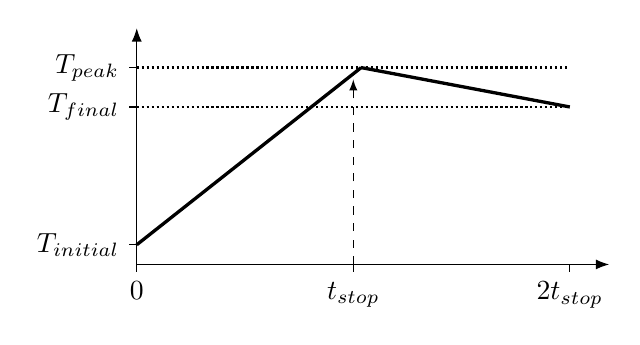
\begin{tikzpicture}
    \draw[-Latex] (0,0) -- (6,0);
    \draw (0,0)    -- (0,-0.1)    node[below] {$0$};
    \draw (2.75,0) -- (2.75,-0.1) node[below] {$t_\text{stop}$};
    \draw (5.5,0)  -- (5.5,-0.1)  node[below] {$2t_\text{stop}$};
    %
    \draw[-Latex] (0,0) -- (0,3);
    \draw (0,0.25)    -- (-0.1,0.25)    node[left] {$T_\text{initial}$};
    \draw (0,2.5)    -- (-0.1,2.5)      node[left] {$T_\text{peak}$};
    \draw[thick, densely dotted] (0,2.5) -- (5.5,2.5);
    \draw (0,2)    -- (-0.1,2)          node[left] {$T_\text{final}$};
    \draw[thick, densely dotted] (0,2) -- (5.5,2);
    %
    \draw[very thick] (0,0.25) -- (2.85,2.5);
    \draw[very thick] (2.85,2.5) -- (5.5,2);
    %
    \draw[dashed, -latex] (2.75,0) -- (2.75,2.35);
\end{tikzpicture}
        \captionof{figure}{Expected time dependence of the temperature of the aluminum cylinder in this experiment. \label{fig: temp vs time}}
    \end{minipage}}
    
    As usual, include the title and axis labels (with units) in your plot to receive full credit.\\[1em]

    \begin{center}
        \captionsetup{font=normalsize}
        \captionof{graph}{Temperature vs. time. \label{graph: mechequiv}}
        
\begin{tikzpicture}
            % Define dimensions
            \def\gridwidth{25}
            \def\gridheight{20}
            \def\spacing{0.6}
            % Draw grid paper on the left
            \begin{scope}[xshift=0cm,yshift=0cm]
                % Major grid lines (thicker)
                \foreach \x in {0,1,...,\gridwidth}
                    \draw[gray!50,thick] (\x*\spacing,0) -- (\x*\spacing,\gridheight*\spacing);
                \foreach \y in {0,1,...,\gridheight}
                    \draw[gray!50, thick] (0,\y*\spacing) -- (\gridwidth*\spacing,\y*\spacing);
                \draw[black, very thick] (0,0) rectangle (\gridwidth*\spacing,\gridheight*\spacing);
            \end{scope}
        \end{tikzpicture}
    \end{center}

    \filbreak
    \question[1] The peak temperature in your graph may not be exactly the same as the temperature when you stopped cranking. Why might it be possible for the temperature reading to rise a bit more after you stop putting energy into the system?
    %
    \begin{solution}[1.5cm]
        
    \end{solution}

    \filbreak
    \question
    \begin{parts}
        \part[\half] Using eq.~\ref{eq: total work}, calculate the work done, $W$, to lift the mass while cranking.
        
        \begin{align*}
            &\text{Total number of revolutions:}     & N&= \uline{\qquad\qquad\qquad\qquad} &
            \\[1em]
            &\text{Mass you lifted off the ground:}  & M&= \uline{\qquad\qquad\qquad\qquad}~\qty{}{\kilo\gram} &
            \\[1em]
            &\text{Mass of the aluminum cylinder:}   & m&= \uline{\qquad\qquad\qquad\qquad}~\qty{}{\kilo\gram} &
            \\[1em]
            &\text{Radius of the aluminum cylinder:} & R&= \uline{\qquad\qquad\qquad\qquad}~\qty{}{\meter} &
        \end{align*}
        %
        \begin{solution}[1cm]
            
        \end{solution}
        %
        \part[\half] Compute the change in temperature $\Delta T = T_\text{peak} - T_\text{initial}$.
        \begin{solution}[1.5cm]
            
        \end{solution}
        %
        \part[\half] Using eqs.~\ref{eq: heat} and \ref{eq: specific heat}, calculate the heat $Q$ you added to the system by raising its temperature $\Delta T$:
        \begin{solution}[1.5cm]
            
        \end{solution}
        %
        \part[\half] Finally, use eq.~\ref{eq: joule's constant measured} to estimate Joule’s constant. Don't forget units.
        \begin{solution}[1.5cm]
            
        \end{solution}
    \end{parts}

    \filbreak
    \question[1] In this experiment, the aluminum cylinder loses heat to the environment because it is hotter than its surroundings. Calculate how much heat was lost after you stopped cranking, $\Delta T_\text{lost}=T_\text{peak}-T_\text{final}$.
    %
    \begin{solution}[1.5cm]
        
    \end{solution}

    \filbreak
    \question[2] While you were still cranking the cylinder, heat was also being lost to the environment because the cylinder was hotter than its surroundings (although less hot than $T_\text{peak}$). If we tried to correct for this in our calculation of Joule’s constant by saying that the total change in temperature due to your cranking should have been $\Delta T + \Delta T_\text{lost}$, why might this overestimate the actual heat lost while cranking?
    %
    \begin{solution}[1.5cm]
        
    \end{solution}

    \filbreak
    \question[2] Discuss one major source of error in this experiment besides the ambient/radiant cooling, and how it may have affected the measured Joule’s constant. 
    Had that error been removed, would it have increased the measured Joule’s constant or decreased it? Explain.
    %
    \begin{solution}[1.5cm]
        
    \end{solution}

\endgradingrange{mechequiv}

\end{postlab}

\end{document}